\documentclass{article}
\usepackage[utf8]{inputenc}
\usepackage{mathtools,amsmath,graphicx,empheq,slashed,color,hyperref}
\usepackage{geometry}
\hypersetup{colorlinks=true,linkcolor=blue,urlcolor=cyan,citecolor=red}
\setlength{\unitlength}{1mm}

\newcommand{\n}{\nonumber \\}
\newcommand{\U}{\mathcal{U}}
\newcommand{\du}{d_\mathcal{U}}
\newcommand{\oo}{\mathcal{O}}
\newcommand{\epem}{e^+e^-}
\newcommand{\nn}{\nonumber}
\newcommand{\hreff}[1]{\href{mailto:#1}{#1}}
\author{Le Van Dung}
\date{ }
\title{Mid term}
\begin{document}
\begin{figure}[h!]
 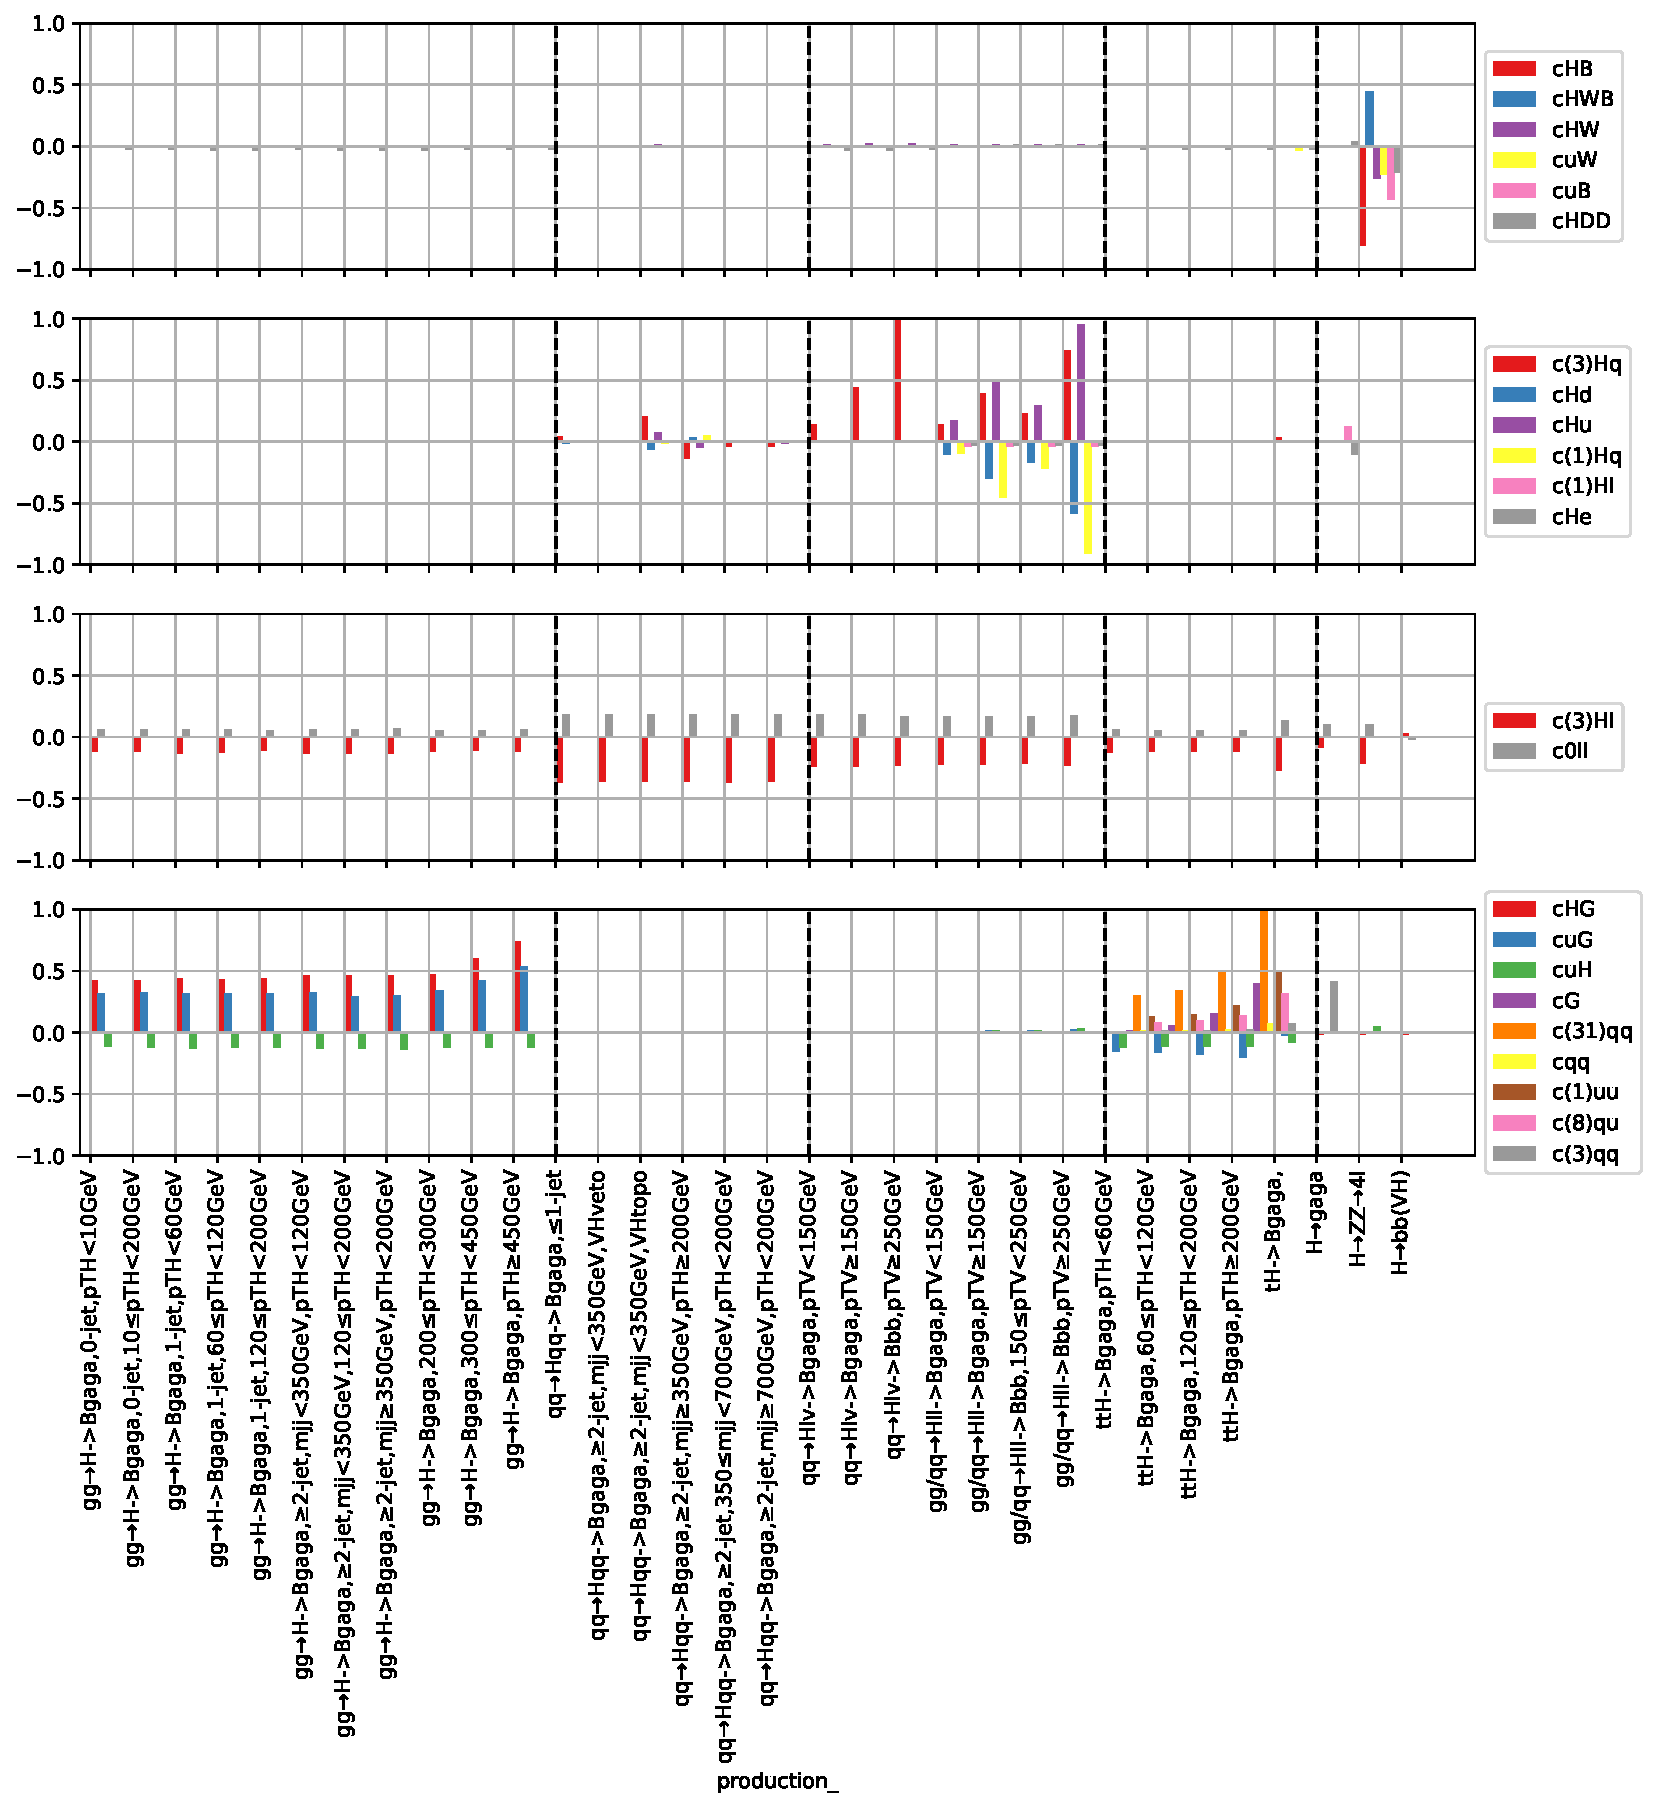
\includegraphics[scale=0.4]{../parameter.pdf}
\end{figure}
\begin{figure}[h!]
 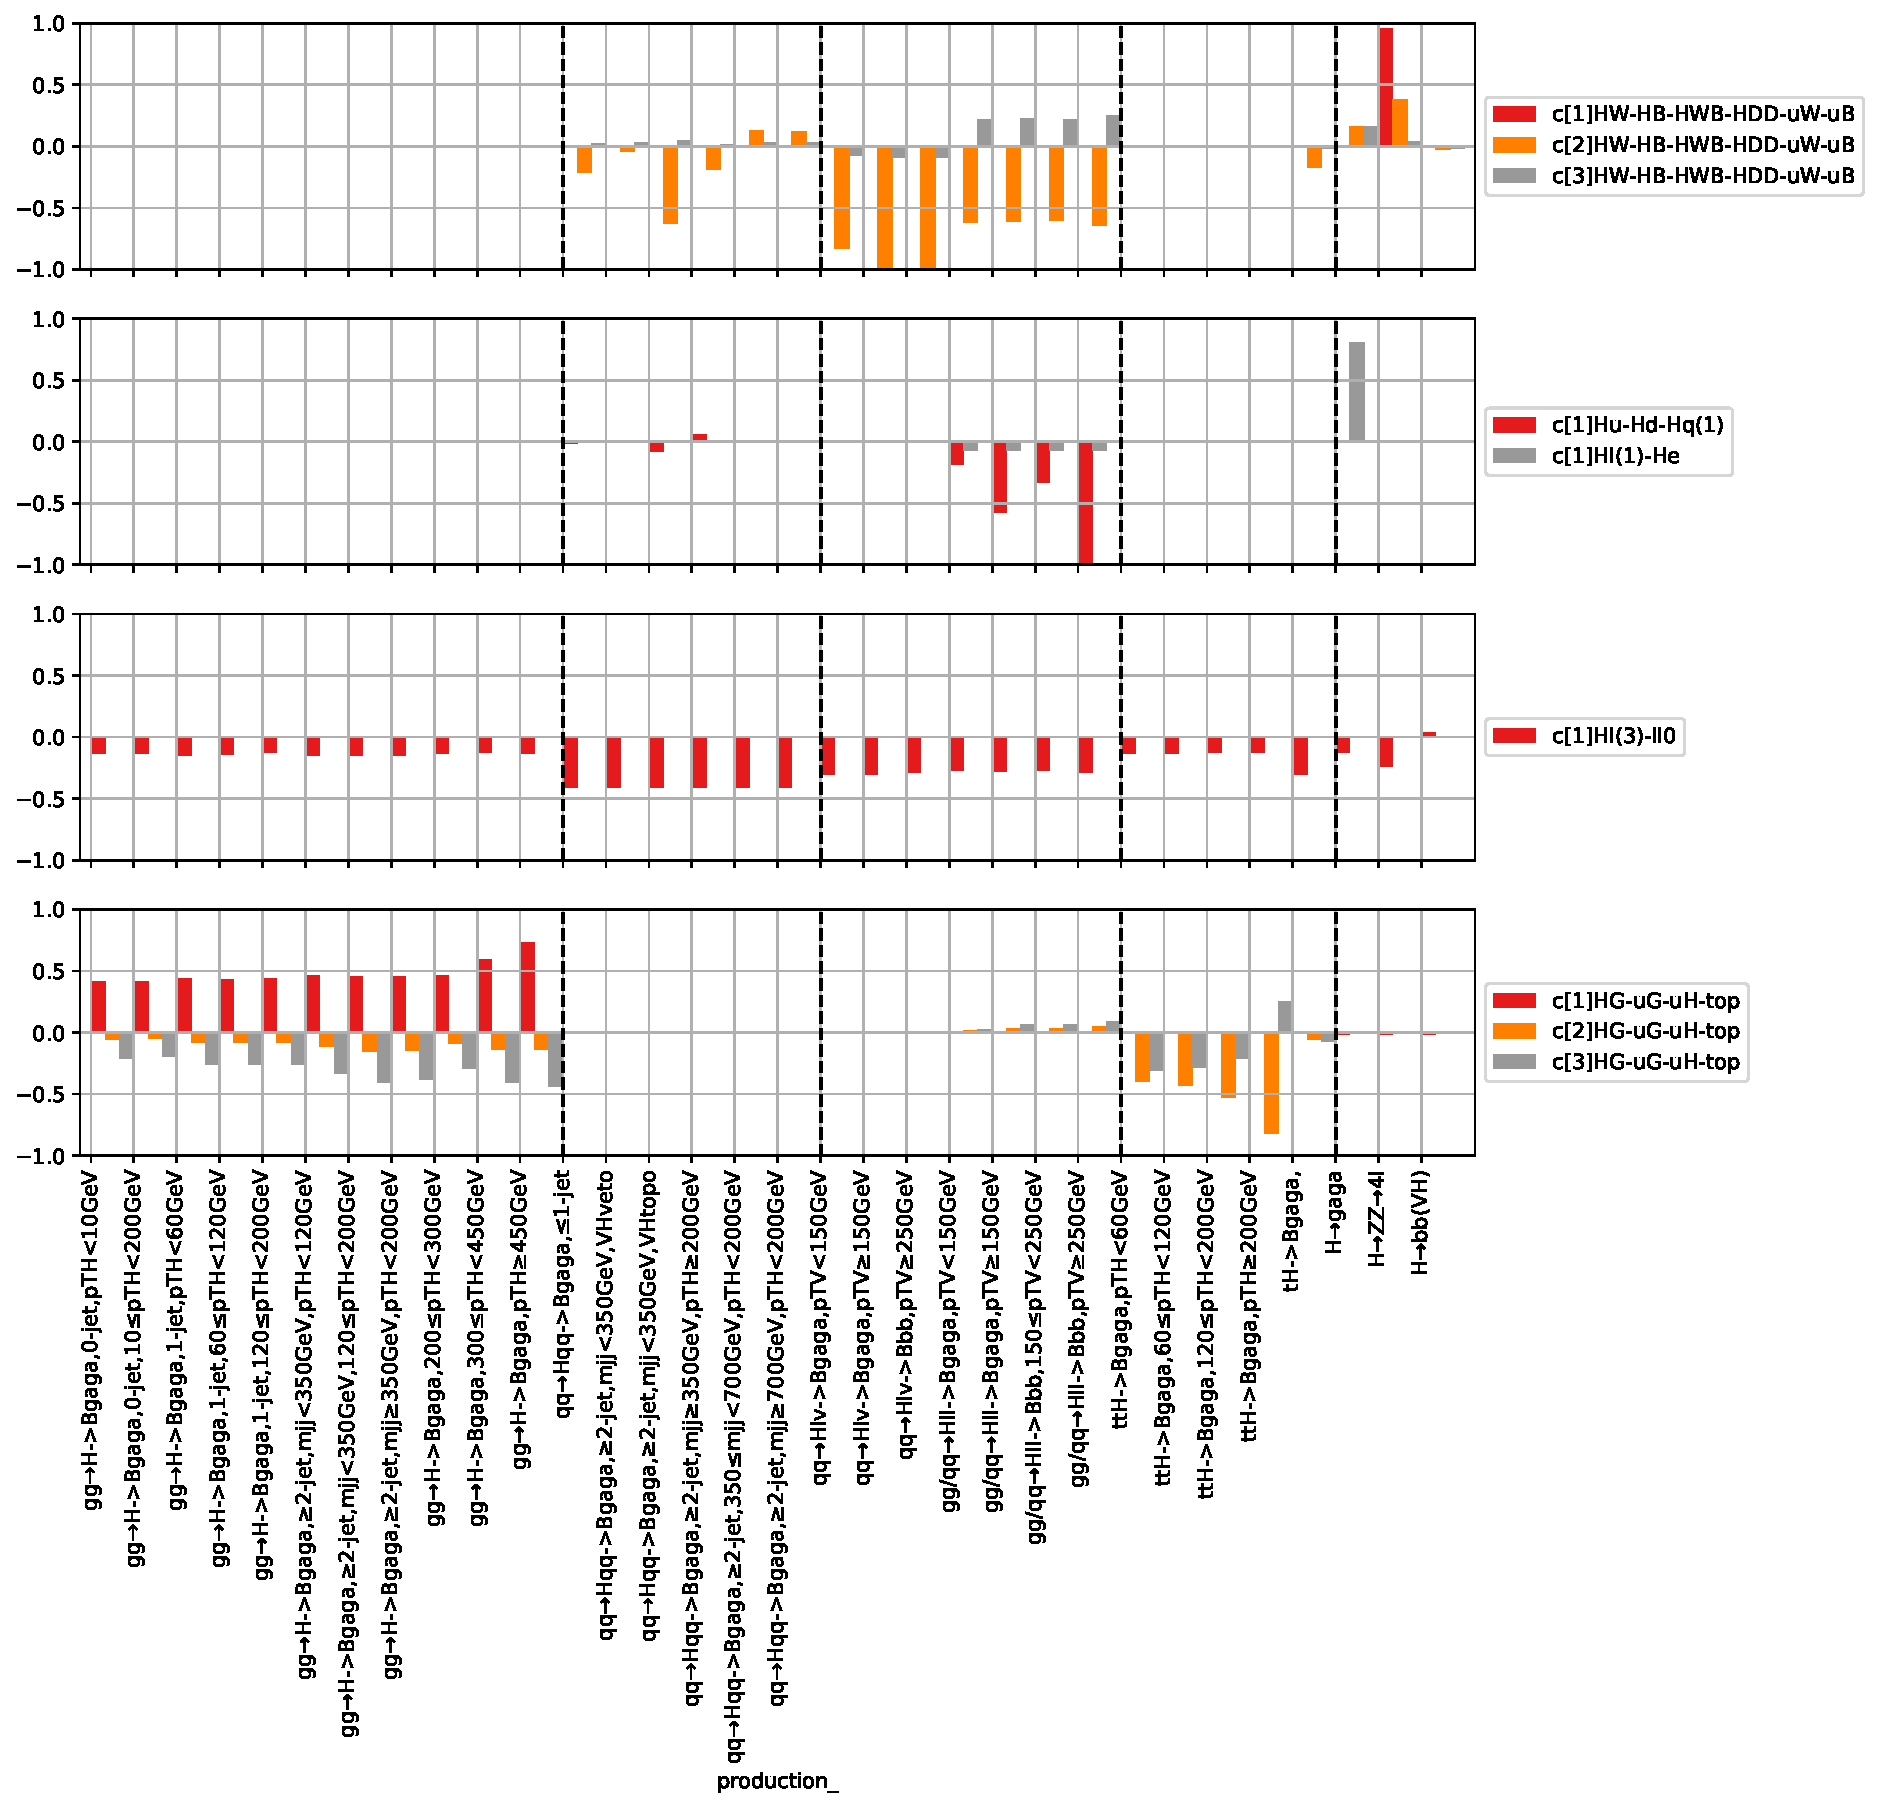
\includegraphics[scale=0.4]{../rotated_parameter.pdf}
\end{figure}
\begin{figure}[h!]
 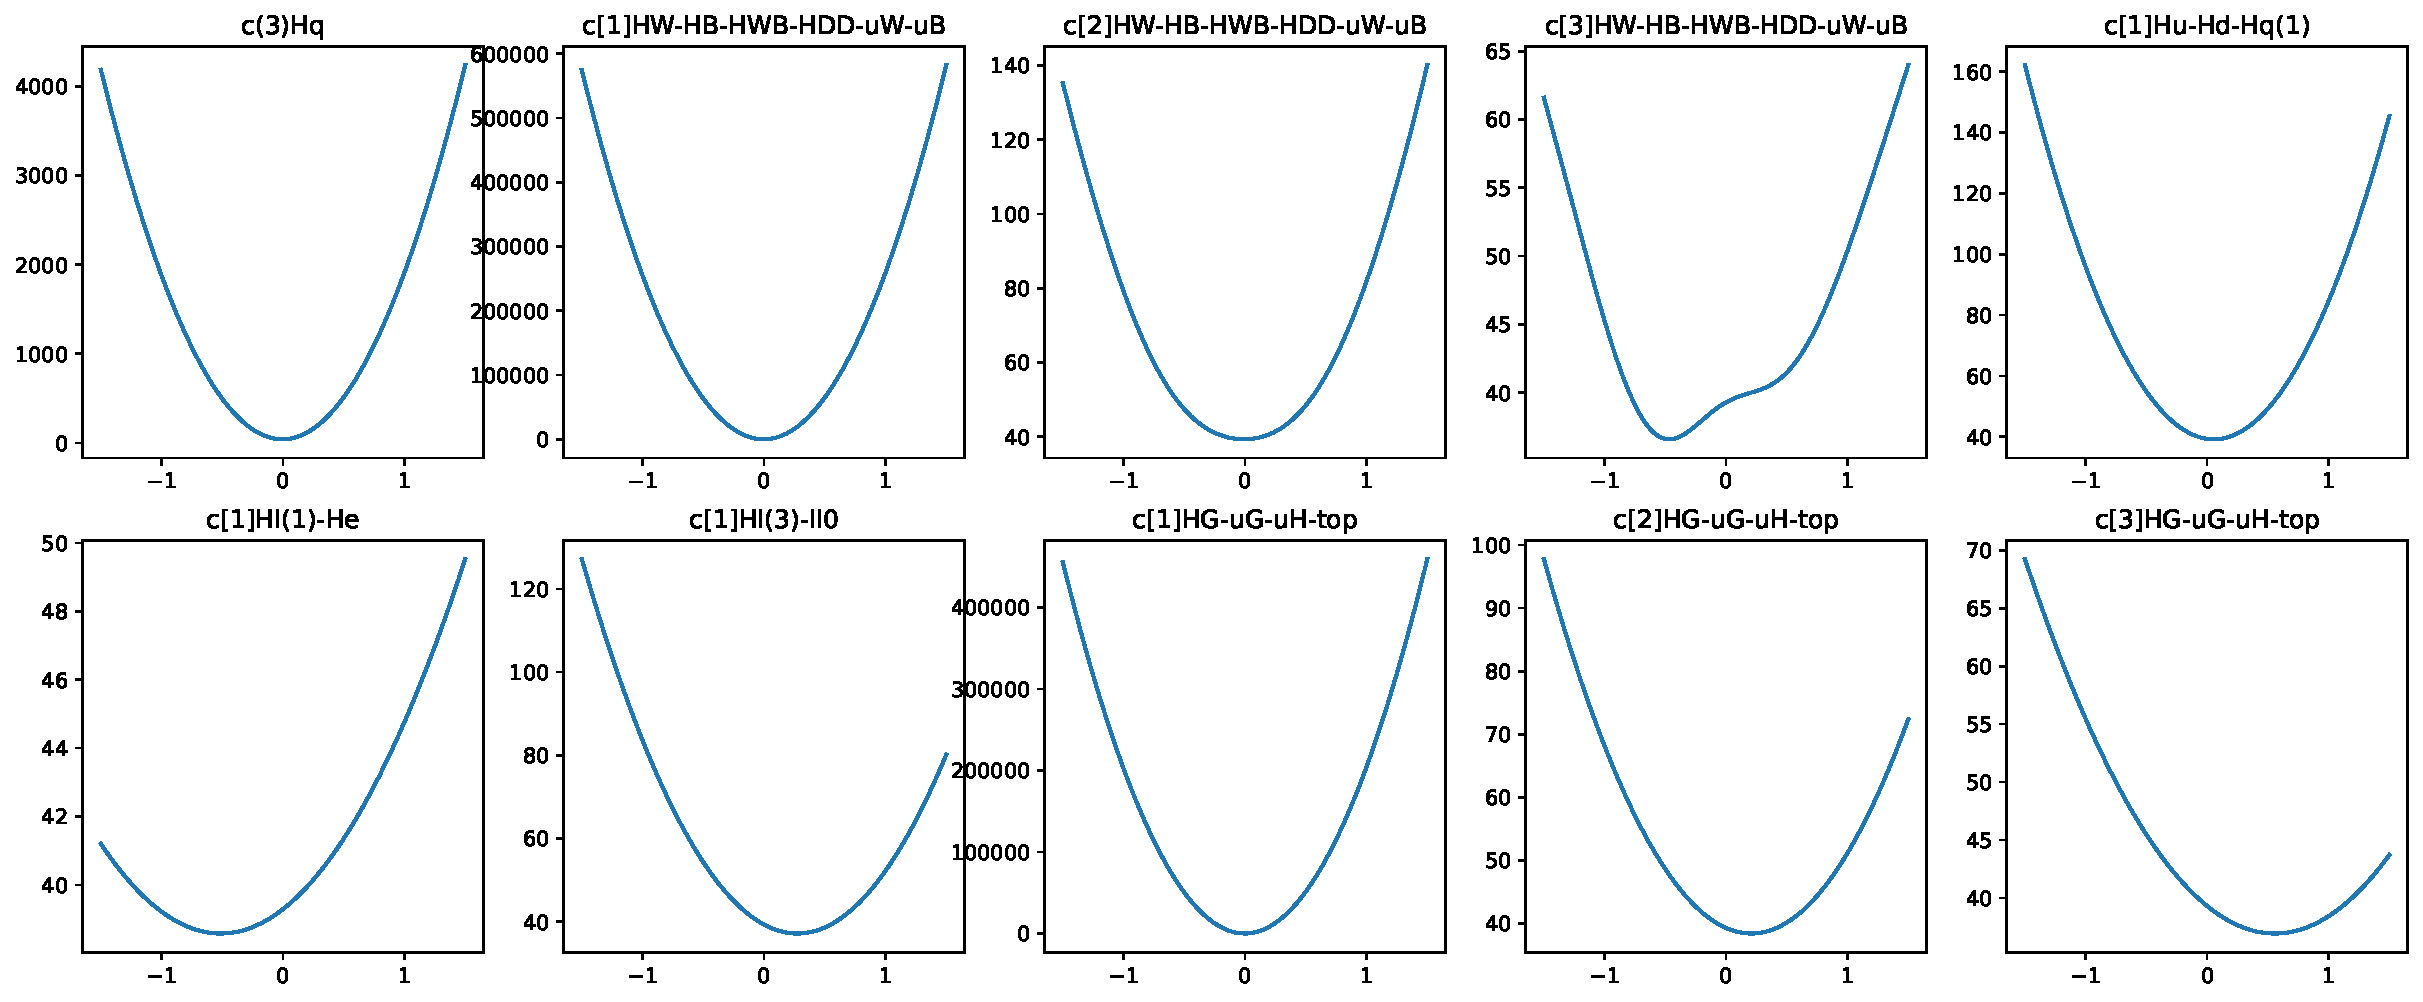
\includegraphics[scale=0.4]{../rotated_parameter_guess.pdf}
 \caption{first scan with every other parameters are set to 0}
\end{figure}
\clearpage
After finding a good scan range, I begin to scan through every $c'_i$ in a specific range and update the minimum value each scan, as the figure below \ref{likelihood}
\begin{figure}[h!]
 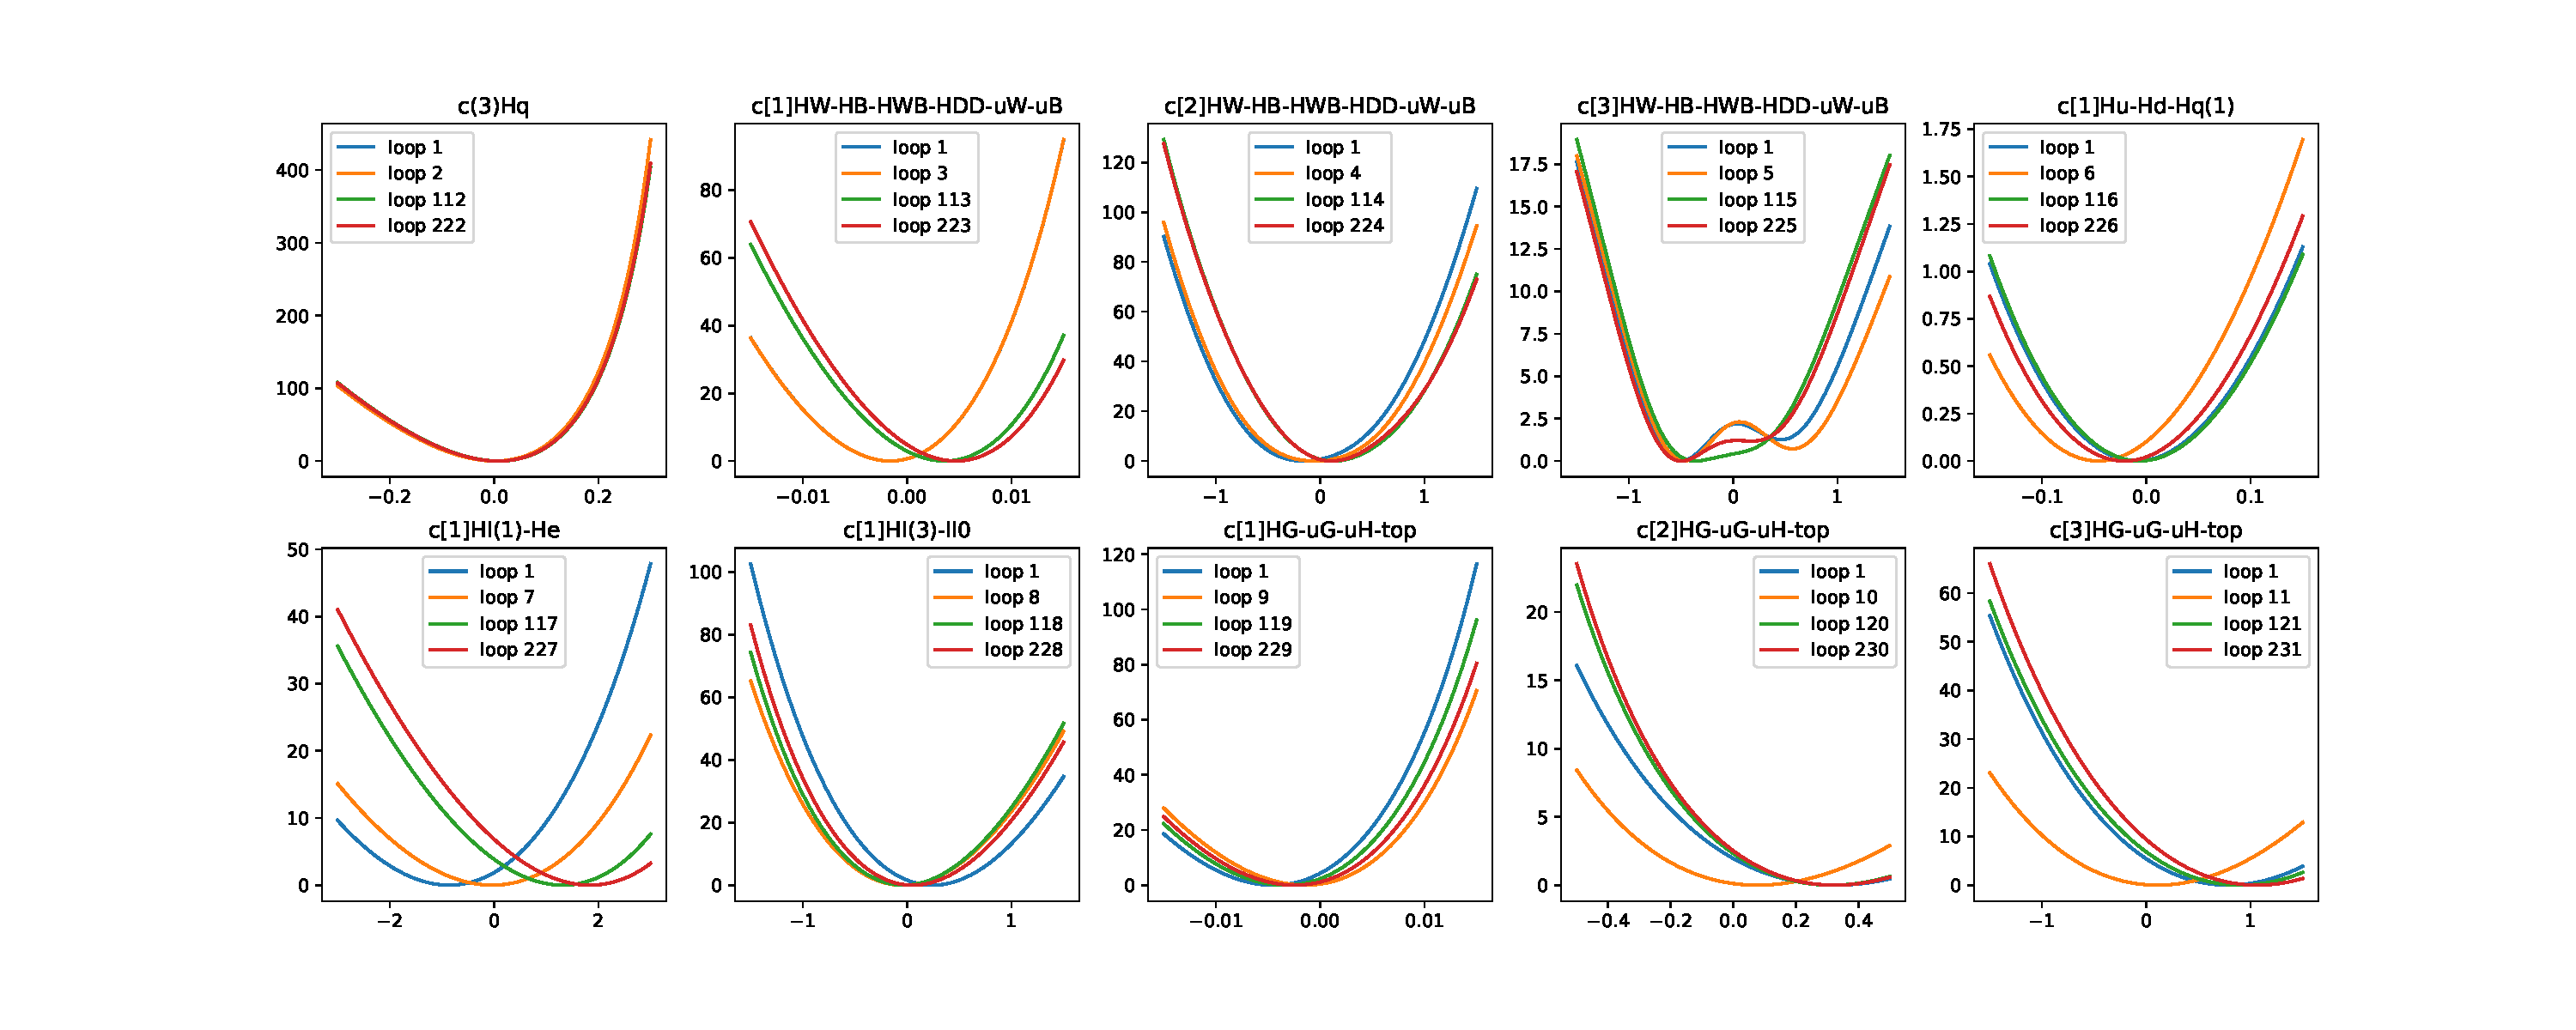
\includegraphics[scale=0.35]{../likelihood.pdf}
 \caption{plot of negative likelihood, for each plot, only relevent coefficient is scanned, others are fixed\label{likelihood}}
\end{figure}
\end{document}